
\chapter{导数与微分}
\section{导数的定义}
\subsection{某点导数的基本定义}
\vspace*{-1em}

\defination[导数定义1]
设函数$y=f(x)$在点$x_{0}$的某一邻域内有定义,当自变量$x$在$x_{0}$取得增量$\Delta x$(点$x_0+\Delta x$仍在该邻域内)时,相应地,因变量取得增量$\Delta y=f(x_0+\Delta x)-f(x_0)$;如果$\Delta y$与$\Delta x$之比当$\Delta x$ $\to$0时的极限存在,那么称函数$y=f(x)$在点$x_0$处\highlight{red}{可导},并这个极限为函数$y=f(x)$\highlight{red}{在$x_0$点的导数\index{DS@导数}},记为$f'(x_0)$,即
\begin{equation}
	f'(x_0)=\lim\limits_{\Delta x\to 0}\frac{\Delta y}{\Delta x}=\lim\limits_{\Delta x\to 0}\frac{f(x_0+\Delta x)-f(x_0)}{\Delta x}
\end{equation}
也可记作:
\begin{equation}
	y'|_{x=x_0} \quad \mbox{或} \quad \frac{\d y}{\d x}\bigg|_{x=x_0}\quad \mbox{或} \quad \frac{\d f(x)}{\d x}\bigg|_{x=x_0}
\end{equation}
\hspace*{2em} 由于在以后的证明中很少用到函数极限定义证明,以下仅给出几道较典型的例题。\\
\hspace*{2em} 在这些例题中有很多运用到了三角公式(可以在附章查阅)和等价无穷小的知识。

\example[用函数极限定义证明以下函数的导数] \vspace*{-1em}
\examples 用函数极限定义证明以下函数的导数\vspace{0.8em} \\
1.\enspace$f(x)=C$($C$为常数)\vspace{0.8em}\\ 
\solve $f'(x)=\lim\limits_{h\to 0}\di \frac{f(x+h)-f(x)}{h}$=$\lim\limits_{h\to 0}$ $\di\frac{C-C}{h}=0$,即
\vspace*{-0.5em}
\begin{equation}
	\nonumber
	f'(x)=(C)'=0
\end{equation}
2.\enspace$f(x)=x^{\mu}$($\mu \in R$)
\vspace{0.8em} \\ \solve $f'(x)=\lim\limits_{h\to 0} \di\frac{f(x+h)-f(x)}{h}=\lim\limits_{h\to 0}\di\frac{(x+h)^{\mu}-x^\mu}{h}=x^{\mu-1}\cdot \lim\limits_{h\to 0}\frac{(1+\frac{h}{x})^\mu-1}{\frac{h}{x}}\\
\hspace*{7em}=x^{\mu-1}\cdot\lim\limits_{h\to 0}\frac{\textstyle \mu\cdot\frac{h}{x}}{\textstyle \frac{h}{x}}=\mu x^{\mu-1}$\vspace{0.8em}\\即
\begin{equation}
	\nonumber
	f'(x)=(x^\mu)'=\mu x^{\mu-1}
\end{equation}
\newpage                                                                 
\noindent 3.\enspace$f(x)=\sin x$
\vspace{0.8em} \\ \solve $f'(x)=\lim\limits_{h\to 0}\di\frac{f(x+h)-f(x)}{h}=\lim\limits_{h\to 0}\di\frac{\sin (x+h)-\sin x}{h}=\lim\limits_{h\to 0}\di\frac{1}{h}\cdot 2\cos\di\bigg(x+\frac{h}{2}\bigg)\cdot\sin\di\frac{h}{2}$\\  
\hspace*{7em} $=\lim\limits_{h\to 0}\frac{\di\sin\frac{h}{2}}{\di\frac{h}{2}}\cdot\cos\bigg(x+\di\frac{h}{2}\bigg)\cdot\di\sin\frac{h}{2}=\cos x$
\\即
\vspace{0.8em}
\begin{equation}
	\nonumber
	f'(x)=(\sin x)'=\cos x
	\vspace*{0.5em}
\end{equation}
4.\enspace$f(x)=a^x(a>0,a\neq1)$
\vspace{0.8em} \\ \solve
$f'(x)=\lim\limits_{h\to 0}\di \frac{f(x+h)-f(x)}{h}=\lim\limits_{h\to0}\frac{a^{x+h}-a^x}{h}=a^x\cdot\lim\limits_{h\to0}\frac{a^h-1}{h}=a^x\cdot\lim\limits_{h\to0}\frac{h\cdot \ln a}{h}=\ln a\cdot a^x$\\
即
\vspace*{0.5em}
\begin{equation}
	\nonumber
	f'(x)=(a^x)'=a^x\cdot\ln a
	\vspace*{0.5em}
\end{equation}
5.\enspace$f(x)=\log_a x(a>0,a\neq1)$
\vspace{0.8em} \\ \solve $f'(x)=\lim\limits_{h\to0}\di\frac{f(x+h)-f(x)}{h}=\lim\limits_{h\to0}\di\frac{\log_a (x+h)-\log_a x}{h}=\lim\limits_{h\to0}\di\frac{1}{h}\cdot\log_a\bigg(1+\di\frac{h}{x}\bigg)=\di\frac{1}{h}\cdot\lim\limits_{h\to0}\di\frac{x}{h}\cdot\log_a\bigg(1+\di\frac{h}{x}\bigg)$\\
令$u=\di\frac{h}{x},h\to0,u\to0$,得
\begin{equation}
	\nonumber f'(x)=\frac{1}{x}\cdot\lim\limits_{h\to0}\frac{x}{h}\cdot\log_a\bigg(1+\frac{h}{x}\bigg)=\frac{1}{x}\cdot\lim\limits_{u\to0}\frac{1}{u}\cdot\log_a(1+u)=\frac{1}{x}\cdot\lim\limits_{u\to0}\log_a(1+u^{\frac{1}{u}})=\frac{1}{x}\cdot\lim\limits_{u\to0}\log_a e=\frac{1}{x}\cdot\frac{1}{\ln a}=\frac{1}{x\cdot\ln a}
	\end{equation}
即
\begin{equation}
	\nonumber
	f'(x)=(\log_a x)'=\frac{1}{x\cdot\ln a}
	\vspace*{0.5em}
\end{equation}
\subsection{导函数与单侧导数}
\vspace*{-1em}

\defination[导数定义2]
如果函数$y=f(x)$在开区间$I$内的每点处都可导,那么就称函数$f(x)$在开区间$I$内可导。这时,对于任意$x\in I$,都对应着$f(x)$的一个确定的导数值。这样就构成了一个新的函数,这个函数叫做原来函数的导函数,简称导数。记作
\begin{equation}
	\nonumber
	f'(x)\quad \mbox{或} \quad y'\quad \mbox{或} \quad \frac{\d y}{\d x}\quad \mbox{或} \quad \frac{\d f(x)}{\d x}
\end{equation} 
则$f(x)$在$x_0$处的导数也可表示为
\begin{equation}
	f'(x_0)=f'(x)|_{x=x_0}
\end{equation} 
\vspace{-2em}
\warn[\hspace*{2em} $f'(x)$是导函数,也就是说$f'(x)$是函数,而$f'(x_0)$是$f(x)$在点$x_0$处的导数或者说$f'(x_0)$是导函数$f'(x)$在$x=x_0$处的值。]
\vspace*{-1em}

\defination[单侧导数]
函数$y=f(x)$在点$x_0$处的\highlight{red}{\index{ZDS@左导数}左导数},\highlight{red}{\index{ZDS@右导数}右导数}分别为
\begin{equation}
	f'_-(x_0)=\lim\limits_{\Delta x\to0^-}\frac{f(x_0+\Delta x)-f(x_0)}{\Delta x} \hspace*{2em} 	f'_+(x_0)=\lim\limits_{\Delta x\to0^+}\frac{f(x_0+\Delta x)-f(x_0)}{\Delta x}
\end{equation}
左导数与右导数统称为\highlight{red}{\index{DCDS@单侧导数}单侧导数}。\\
\hspace*{2em} 函数$y=f(x)$在点$x_0$可导的充分必要条件为\textbf{左导数与右导数存在且相等}。\\
\hspace*{2em} 如果函数$f(x)$在开区间$(a,b)$内可导,且$f'_+(a),f'_-(b)$都存在,那么就说$f(x)$在闭区间$[a,b]$内可导。
\section{利用基本求导法则与导数公式求函数的导数}
\subsection{几个补充的函数}\vspace*{0.5em}
\noindent 1.\enspace 双曲函数与反双曲函数\vspace*{1em}\\
双曲正弦函数 \hspace*{2em} sh $x=\di\frac{e^x-e^{-x}}{2}$  \hspace*{2em} \hspace*{2em} 反双曲正弦函数\hspace*{2em} arsh $x=\ln(x+\sqrt{x^2+1})$\vspace*{1em}\\
双曲余弦函数 \hspace*{2em} ch $x=\di\frac{e^x+e^{-x}}{2}$  \hspace*{2em} \hspace*{2em} 反双曲余弦函数\hspace*{2em} arch $x=\ln(x\pm\sqrt{x^2+1})\left\{\begin{aligned}
		&  \, x>0:+\\
		&  \, x<0:-\\
		\end{aligned}\right.
		$\vspace*{1em}\\
双曲正切函数 \hspace*{2em} th $x=\di\frac{e^x-e^{-x}}{e^x+e^{-x}}$  \hspace*{2em} \hspace*{2em} 反双曲正切函数\hspace*{2em} arth $x=\di\frac{1}{2}\ln\di\frac{1+x}{1-x}$\vspace*{1em}\\
2.\enspace 三角函数的补充函数\vspace*{1em}\\
余割函数 \hspace*{2em} csc $x=\di\frac{1}{\sin x}$  \hspace*{2em} \hspace*{2em} 正割函数\hspace*{2em} sec $x=\di\frac{1}{\cos x}$\vspace*{1em}\\
余切函数 \hspace*{2em} cot $x=\di\frac{1}{\tan x}$  \hspace*{2em} \hspace*{2em} 反三角函数\hspace*{2em}  $\arcsin x$,$\arccos x$,$\arctan x$,arccsc $x$,arcsec $x$,arccot $x$
\subsection{基本函数的求导公式}\vspace*{-3em}
\begin{flalign*}
 \qquad & 1.\enspace(C)'=0(C\text{为常数})   && 2.\enspace(x^\mu)'=\mu x^{\mu-1}\vspace{1em}&&\\
\qquad & 3.\enspace(\sin x)'=\cos x   & &4.\enspace(\cos x)'=-\sin x\vspace{1em}&&\\
\qquad & 5.\enspace(\tan x)'=\text{sec}^2 x   && 6.\enspace(\cot x)'=-\csc^2 x\vspace{1em}&&\\
\qquad & 7.\enspace(\sec x)'=\sec x\cdot\tan x   && 8.\enspace(\csc x)'=-\csc x\cdot \tan x\vspace{1em}&&\\
\qquad & 9.\enspace(a^x)'=a^x\cdot\ln a(a>0,a\neq1)   &&10.\enspace(\log_a x)'=\frac{1}{x\cdot\ln a}(a>0,a\neq1)\vspace{1em}&&\\
\qquad & 11.\enspace(\arcsin x)'=\frac{1}{\sqrt{1-x^2}}   & &12.\enspace(\arccos x)'=-\frac{1}{\sqrt{1-x^2}}\vspace{1em}&&\\
\qquad & 13.\enspace(\arctan x)'=\frac{1}{1+x^2}   
\qquad & &14.\enspace(\text{arccot}\hspace{0.2em} x)'=-\frac{1}{1+x^2}\vspace{1em}&&\\
\qquad &15.\enspace(\text{ch}\hspace{0.2em} x)'=\text{sh}\hspace{0.2em} x   & &16.\enspace(\text{sh}\hspace{0.2em} x)'=\text{ch}\hspace{0.2em} x\vspace{1em}&&\\
\qquad &17.\enspace(\text{th}\hspace{0.2em}x)'=\frac{1}{\text{ch}^2x}&
\end{flalign*}
\subsection{函数求导法则}
设$f(x),g(x)$可导,则
\begin{flalign*}
\qquad &1.\enspace[f(x)+g(x)]'=f'(x)+g'(x) &2.&\enspace[Cf(x)]'=Cf'(x)(C\text{为常数})\vspace{1em}&&\\[0.5em]
\qquad &3.\enspace[f(x)\cdot g(x)]'=f'(x)\cdot g(x)+f(x)\cdot g'(x) &4.&\enspace\bigg[\frac{f(x)}{g(x)}\bigg]'=\frac{f'(x)\cdot g(x)-f(x)\cdot g'(x)}{[g(x)]^2}&&
\end{flalign*}
\subsection{反函数的求导法则}
设$x=f(y)$在区间$I_y$内单调、可导且$f'(y)$,则它的反函数$y=f^{-1}(x)$在$I_x=f(I_y)$内也可导,则
\begin{equation}
	[f^{-1}(x)]'=\frac{1}{f'(y)}\quad \mbox{或} \quad \frac{\d y}{\d x}=\frac{1}{\di\frac{\d x}{\d y}}
\end{equation}
\subsection{复合函数的求导法则}
设$y=f(u),u=g(x)$,且$f(u),g(x)$都可导,则复合函数$y=f[g(x)]$的导数为;
\begin{equation}
	\frac{\d y}{\d x}=\frac{\d y}{\d u}\cdot\frac{\d u}{\d x}\quad \mbox{或} \quad y'(x)=f'(u)\cdot g'(x)
\end{equation}
\section{函数的微分}
\subsection{微分的定义}
\vspace{-0.5em}
\defination[微分的定义]
设函数$y=f(x)$在某区间内有定义$x_0$,及$x_0+\Delta x$在这区间内,如果函数的增量
\begin{equation}
	\Delta y=f(x_0+\Delta x)-f(x)
\end{equation}
表示为:
\begin{equation}
	\Delta y=A\Delta x+o(\Delta x)
\end{equation}
其中$A$是不依赖于$\Delta x$的常数,那么称函数$y=f(x)$在点$x_0$处是\highlight{red}{可微}的,而$A\Delta x$叫做函数在点$x_0$相应于自变量增量$\Delta x$的\highlight{red}{\index{WF@微分}微分},记作$
\d y$,即:
\begin{equation}
	\d y=A\Delta x
\end{equation}
\hspace*{2em} 函数$y=f(x)$在点$x_0$处可微的充分必要条件是函数$y=f(x)$在点$x_0$可导,且当$f(x)$在点$x_0$可微时,其微分一定是
\begin{equation}
	\d y=f'(x_0)\Delta x
\end{equation}
当$\Delta x\to 0$时,有
\begin{equation}
	\lim\limits_{\Delta x\to 0}\frac{\Delta y}{\d y}=\lim\limits_{\Delta x\to 0}\frac{\Delta y}{f^{'}(x_0)\Delta x}=\frac{1}{f^{'}(x_0)}\lim\limits_{\Delta x\to 0}\frac{\Delta y}{\Delta x}=\frac{1}{f^{'}(x_0)}f'(x_0)=1\vspace*{0.5em}
\end{equation} 
从而,当$\Delta x\to 0$时,$\Delta y$与$\d y$是等价无穷小,于是这时有
\begin{equation}
	\Delta y=\d y+o(\d y)
\end{equation}

即$\d y$是$\Delta y $的主部\footnote{设$\alpha$,$ \beta$ 都是在同一个自变量的变化过程中的无穷小,如果$\beta=\alpha +o(\alpha)$,则称$\alpha$是$\beta$的主部.},又由于$\d y=f'(x_0)\Delta x$是$\Delta x$的线性函数。所以在$f'(x_0)\neq0$的条件下,我们说$\d y$是$\Delta x$的线性主部(当$\Delta x\to 0$时)。于是我们得到以下结论:
\\  \hspace*{2em} 在$f'(x_0)\neq0$的条件下,以微分$\d y=f'(x_0)\Delta x$近似代替增量$\Delta y=f(x_0+\Delta x)-f(x_0)$时,其误差为$o(\d y).$
\subsection{微分的几何意义}
如图 \ref{微分几何意义} 所示,在直角坐标系中,函数$y=f(x)$的图形是一条曲线相对与某一固定的$x_0$值,曲线上有一个确定点$M(x_0,y_0)$,当自变量$x$有微小增量$\Delta x$时,就得到曲线上另一点$N(x_0+\Delta x,y_0+\Delta y)$,

\noindent
\begin{minipage}{0.45\linewidth}
\qquad 从图 \ref{微分几何意义} 可知,
	\begin{equation}
	\nonumber
	MQ=\Delta x=\d x,NQ=\Delta y
\end{equation}
过点$M$作曲线的切线$MT$,它的倾角为$\alpha$,则
\begin{equation}
	\nonumber
	QP=MQ\cdot \tan\alpha=\Delta x\cdot f'(x_0)
\end{equation}
即
\begin{equation}
	\nonumber
	\d y=QP
\end{equation}
\end{minipage}
\begin{minipage}{0.55\linewidth}
	\centering
	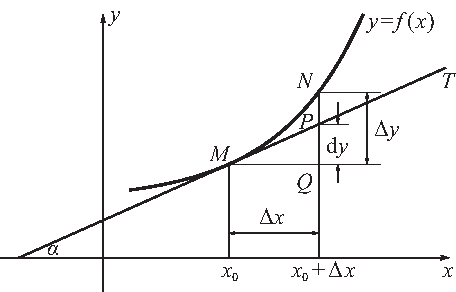
\includegraphics[width = 0.8\linewidth]{pic/C-2/微分几何意义.pdf}
	\vspace*{-1em}
	\captionof{figure}{微分的几何意义}
	\label{微分几何意义}
\end{minipage}
\vspace*{1.5em}

\myitem{$\bullet${\normalsize\textbf{微分的几何意义的应用}}\vspace{0.2em}\\
\hspace*{2em} 对于可微函数$y=f(x)$而言,当$\Delta y$是曲线$y=f(x)$上的点的纵坐标的增量时,$\d y$就是曲线的切线上的点的纵坐标的相应增量,当$|\Delta x|$很小时,$|\Delta y-\d y|$比$|\Delta x|$小得多。因此在点$M$的邻近,我们可以用切线段来近似代替曲线段。在局部范围内用线性函数近似替代非线性函数,在几何上就是局部用切线段近似代替曲线段。这在数学上称为\textbf{非线性函数的局部线性化}。这是微分学的基本思想方法之一。这种思想方法在自然科学和工程问题的研究中是经常采用的。}
\subsection{基本初等函数的微分公式}
从函数的微分表达式
\begin{equation}
	\d y=f'(x)\, \d x\quad \mbox{或} \quad \d f(x)=f'(x)\, \d x
\end{equation}
\hspace*{2em} 可以看出,要计算函数的微分只需要计算函数的导数,再乘以自变量的微分,例如:$\d(\sin x)=\cos x \d x$,其它基本初等函数的微分也类似,故在此不再赘述。(参见基本函数求导公式)
\subsection{微分运算法则}
由函数和差\vspace*{-2.5em}法则,可推得相应的微分法则。
\begin{flalign*}
	\qquad &1.\enspace d(u\pm v)=\d u+\d v &2.&\enspace \d(uv)=v\d u+u\d v&&\\[0.5em]
	\qquad &3.\enspace\d(Cu)=C\d u &4.&\enspace\d\bigg(\frac{u}{v}\bigg)=\frac{v\d u-u\d v}{v^2}&&
\end{flalign*}
设$y=f(u)$及$u=g(x)$都可导,则复合函数$y=f[g(x)]$的微分为
\begin{equation}
	\d y=y'_x\,\d x=f'(u)g'(x)\,\d x
\end{equation}
由于$g(x)\,\d x=\d u$,所以,复合函数$y=f[g(x)]$的微分公式也可以写成
\begin{equation}
\d y=f'(u)\,\d u\quad \mbox{或} \quad \d y=y'_u\,\d u
\end{equation}
\hspace*{2em} 由此可见,无论$u$是自变量还是中间变量。微分形式$\d y=f'(u)\,\d u$保持不变。这一性质称为微分形式不变性,这性质表明,当变换自变量时,微分形式$\d y=f'(u)\,\d u$并不改变。
\clearpage

\vspace*{-2.5em}
\warn[\hspace*{2em} 微分形式不变性仅适用于一阶微分,对于二阶及以上的微分并不成立,这个在高阶导数和高阶微分中会详细说明。]
\section{隐函数的导数}
\subsection{隐函数与显函数的概念}
\defination[显函数定义]
等号左端是因变量的符号,而右端是含有自变量的式子,当自变量取定义域内任一值时,由这式子能确定对应的函数值。用这种方式表达的函数叫做\highlight{red}{\index{XHS@显函数}显函数},例:$y=x^3+3x^2+x+1,y=\sin x,y=\ln x+\sqrt{1-x^2}.$

\defination[隐函数定义]
一般地,如果变量$x$和$y$满足一个方程$F(x,y)=0$,在一定条件下,当$x$取某区间的任一值时,相应地总有满足这方程的唯一的$y$值存在,那么就说方程$F(x,y)=0$在该区间内确定了一个\highlight{red}{\index{YHS@隐函数}隐函数}。把一个隐函数化成显函数,叫做\highlight{red}{\index{YHSDXH@隐函数的显化}隐函数的显化}。例:$x^2+y^3-1=0,e^{xy}+x+y-2=0.$
\subsection{隐函数的导数}
对于任意一个隐函数$F(x,y)=0$,对其求导,只需两边同时对$x$求导,即
\begin{equation}
	\frac{\d}{\d x}[F(x,y)]=0
\end{equation}
其中需要注意的是,由于$y$是$x$的因变量,所以在求导的过程中$y$要看成$f(x)$来求导,即
\begin{equation}
\frac{\d}{\d x}y=\frac{\d y}{\d x}=y'=f'(x)
\end{equation}
\examples 求由方程$e^y+xy-e=0$所确定的隐函数的导数
\\ \solve 我们把方程两边分别对$x$求导数,方程左边求导得:
\begin{equation}
	\nonumber
\frac{\d}{\d x}(\e^y+xy-\e)=\e^y\frac{\d y}{\d x}+y+x\frac{\d y}{\d x}
\end{equation}
方程左边求导得:
\begin{equation}
	\nonumber
(0)'=0
\end{equation}
所以
\begin{equation}
	\nonumber
	\e^y\frac{\d y}{\d x}+y+x\frac{\d y}{\d x}=0
\end{equation}
即\begin{equation}
	\frac{\d y}{\d x}=-\frac{y}{x+\e^y}(x+\e^y\neq0)
\end{equation}

有些时候对于复杂的显函数也可以用隐函数求导的方法进行求导,常见的方法就是\highlight{red}{\index{DSQDF@对数求导法}对数求导法},下面给出两个典型例题。
\clearpage
\vspace*{-2.5em}

\examples 求函数$y=x^{\textstyle \sin x}$的导数

\solve 等式两边分别取对数,得$\ln y=\sin x\cdot \ln x$\\[0.5em]
我们把方程两边分别对$x$求导数,得
\begin{equation}
	\nonumber
\frac{1}{y}y'=\cos x\cdot \ln x+\sin x\cdot \frac{1}{x}
\end{equation}
即\begin{equation}
	\nonumber
	y'=y\bigg(\cos x\cdot \ln x+\frac{\sin x}{x}\bigg)=x^{\sin x}\bigg(\cos x\cdot \ln x+\frac{\sin x}{x}\bigg)
	\vspace*{1.5em}
\end{equation}

\noindent \examples 求函数$y=\sqrt{\di\frac{(x-1)(x-2)}{(x-3)(x-4)}}$的导数
\\ \solve 等式两边取对数,得
\vspace*{-1em}
\begin{equation}
	\nonumber
	\ln y=\frac{1}{2}[\ln(x-1)+\ln(x-2)-\ln(x-3)-\ln(x-4)]
\end{equation}
我们将方程两边分别对$x$求导数,得
\begin{equation}
	\nonumber
	\frac{1}{y}y'=\frac{1}{2}\bigg(\frac{1}{x-1}+\frac{1}{x-2}+\frac{1}{x-3}+\frac{1}{x-4}\bigg)
\end{equation}
即\begin{equation}
	\nonumber
	y'=\frac{1}{2}y\bigg(\frac{1}{x-1}+\frac{1}{x-2}+\frac{1}{x-3}+\frac{1}{x-4}\bigg)
\end{equation}
\section{由参数方程所确定的函数的导数}
\subsection{参数方程所确定的函数的定义}
\defination[参数方程所确定的函数]
一般地,若\highlight{red}{\index{CSFC@参数方程}参数方程}
\begin{equation}
	\left\{ \begin{aligned}
		&\, x=\varphi(t)\\
		&\, y=\psi (t)\\
	\end{aligned}\right.
\end{equation}
确定$y$与$x$的关系,则称此函数关系所表达的函数为由上述\highlight{red}{参数方程所确定的函数}。
\subsection{参数方程所确定的函数的导数}
\noindent1.\enspace 参数方程的一阶导数
对于一个由下列参数方程所确定的函数
\begin{equation}
	\nonumber
	\left\{ \begin{aligned}
		&\, x=x(t)\\
		&\, y=y (t)\\
	\end{aligned}\right.
\end{equation}
其导数的计算式为
\begin{equation}
	\frac{\d y}{\d x}=\frac{\d y}{\d t}\cdot \frac{\d t}{\d x}=\frac{\d y}{\d t}\cdot\frac{1}{\bigg(\di\frac{\d x}{\d t}\bigg)}=\frac{y'(t)}{x'(t)}
\end{equation}
\clearpage
\vspace*{-1em}
\begin{minipage}{0.57\linewidth}
\examples 已知椭圆的参数方程为
\begin{equation}
	\nonumber
	\left\{ \begin{aligned}
		&\, x=a\cos t\\
		&\, y=b\sin t\\
	\end{aligned}\right.
\end{equation}
	求椭圆在$t=\di\frac{\pi}{4}$相应的点处的切线方程。\\[0.5em]
\solve 当$t=\di\frac{\pi}{4}$时,椭圆上相应的点$M_0$的坐标为
\vspace*{-1.2em}
\begin{equation}
	\nonumber
	\left\{ \begin{aligned}
		&\, x_0=a\cos \frac{\pi}{4}=\frac{\sqrt{2}a}{2}\\[0.5em]
		&\, y_0=b\cos \frac{\pi}{4}=\frac{\sqrt{2}b}{2}\\
	\end{aligned}\right.
\end{equation}
\end{minipage}
\begin{minipage}{0.35\linewidth}
	\centering
	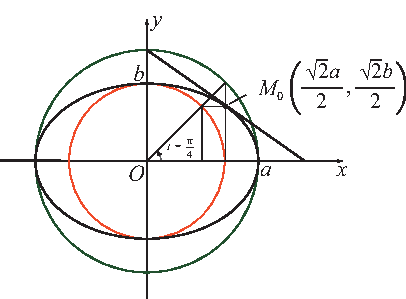
\includegraphics[width=\linewidth]{pic/C-2/椭圆切线}
	\vspace*{-2em}
	\captionof{figure}{椭圆上$t = \dfrac{\pi}{4}$处的切线}
\end{minipage}
\vspace*{1em}

\noindent 曲线在$M_0$的切线斜率为:
\begin{equation}
	\nonumber
	\frac{\d y}{\d x}\bigg|_{t=\frac{\pi}{4}}=\frac{(b\sin t)'}{(a\cos t)'}\bigg|_{t=\frac{\pi}{4}}=\frac{b\cos t}{-a\sin t}\bigg|_{t=\frac{\pi}{4}}=-\frac{b}{a}
\end{equation}
代入点斜式方程,即得椭圆在点$M_0$处的切线方程
\begin{equation}
	\nonumber
	y-\frac{\sqrt{2}}{2}b=-\frac{b}{a}\bigg(x-\frac{\sqrt{2}}{2}a\bigg)
\end{equation}
化简得
\begin{equation}
	\nonumber
	bx+ay-\sqrt{2}ab=0
\end{equation}
2.\enspace 参数方程的二阶导数

对于一个由下列参数方程所确定的函数
\begin{equation}
	\nonumber
	\left\{ \begin{aligned}
		&\, x=x(t)\\
		&\, y=y (t)\\
	\end{aligned}\right.
\end{equation}
其二阶导数的计算式为
\begin{equation}
	\frac{\d^2 y}{\d x^2}=\frac{\d\bigg(\di\frac{\d y}{\d x}\bigg)}{\d x}=\frac{\d\di\bigg(\frac{\d y}{\d x}\bigg)}{\d t}\cdot \frac{\d t}{\d x}=\di\frac{\di\d\bigg[\frac{(\frac{\d y}{\d t})}{(\frac{\d x}{\d t})}\bigg]}{\d t}\cdot \frac{\d t}{\d x}=\bigg(\frac{y^{'(t)}}{x^{'(t)}}\bigg)'\cdot\frac{1}{x^{'(t)}}
\end{equation}
\section{高阶导数与高阶微分}
\subsection{高阶导数的定义}
\defination[高阶导数定义]
一般地,函数$y=f(x)$的导数$f'(x)$叫做函数$y=f(x)$的\highlight{red}{\index{YJDS@一阶导数}一阶导数}。类似地,一阶导数的导数叫做\highlight{red}{\index{EJDS@二阶导数}二阶导数},二阶导数的导数是\highlight{red}{\index{SJDS@三阶导数}三阶导数} $\cdots\cdots$一般地,$(n-1)$阶导数的导数叫做\highlight{red}{$n$阶导数},分别记作
\begin{equation}
	y',y'',y''',\cdots,y^{(n)}\quad \mbox{或} \quad \frac{\d y}{\d x},\frac{\d^2 y}{\d x^2},\frac{\d^3 y}{\d x^3},\cdots,\frac{\d^n y}{\d x^n},
\end{equation}
函数$y=f(x)$具有$n$阶导数,也可以说函数$f(x)$为\highlight{red}{$n$阶可导}。如果函数$f(x)$在点$x$处具有$n$阶导数,那么$f(x)$在点$x$的某一领域内必定有一切低于$n$阶的导数。二阶及二阶以上的导数统称\highlight{red}{\index{GJDS@高阶导数}高阶导数}。
\subsection{一般高阶导数的求法}

\noindent 1.\enspace 多次连续求导;
\\2.\enspace 找到相邻阶导数的关系(递推关系);\\
3.\enspace 利用递推数列的相关解法推出通式,进而写出高阶导数的通式。\\
下面给出一个具体例子\vspace{0.5em}\\
\examples 求函数$y=\sin x$的$n$阶导数
\\ \solve $y'=\cos x=\sin\bigg(x+\di\frac{\pi}{2}\bigg),y''=\cos \bigg(x+\di\frac{\pi}{2}\bigg)=\sin\bigg(x+\di\frac{\pi}{2}+\frac{\pi}{2}\bigg)=\sin\bigg(x+2\cdot\di\frac{\pi}{2}\bigg),\cdots$
我们就可以观察出一定的规律:每求一次导数,三角函数相当于加了$\di\frac{\pi}{2}$角度,即
\begin{equation}
	y^n=\sin\bigg(x+n\cdot\frac{\pi}{2}\bigg)
\end{equation}
\vspace*{-1em}\vspace*{-1em}\vspace*{-1em}
\summarize[\hspace*{2em} 对于一般的函数求其$n$阶导数,都是先求其$1,2,3$阶导函数,找到其中的规律从而写出通式。常见函数$n$阶导函数有:
\begin{equation}
	(a^x)^{(n)}=a^x\cdot\ln^na(a>0,a\neq1)\xrightarrow{\di  a=\e}(\e^x)^{(n)}=\e^x
	\end{equation}
\begin{equation}
	{[(a+bx)^{\mu}]}^{(n)}=
\mu(\mu-1)(\mu-2)\cdots(\mu-n+1)b^n(a+bx)^{\mu-n}
\end{equation}
\begin{equation}
	(\sin x)^n=\sin\bigg(x+n\cdot\frac{\pi}{2}\bigg)
\end{equation}
\begin{equation}
	(\cos x)^n=\cos\bigg(x+n\cdot\frac{\pi}{2}\bigg)
\end{equation}
\begin{equation}
\ln(1+x)^{(n)}=(-1)^{n-1}\frac{(n-1)!}{(1+x)^n}
	\end{equation}
\begin{equation}
	\bigg(\frac{1}{a+bx}\bigg)^{(n)}=(-1)^{n}\frac{n!b^n}{(a+bx)^{n+1}}(b\neq0)
  \end{equation}]
\subsection{函数运算的高阶导数}
\noindent 1.\enspace 加减运算函数的$n$阶导数\\
\hspace*{2em} 设函数$u=u(x),v=v(x)$在点$x$处有$n$阶导数,那么$u(x)+v(x),u(x)-v(x)$在点$x$处也具有$n$阶导数,且
\begin{equation}
	(u\pm v)^{(n)}=u^{(n)}+v^{(n)}
\end{equation}
2.\enspace 乘法运算函数的$n$阶导数
\\ \hspace*{2em} 设函数$u=u(x),v=v(x)$在点$x$处具有$n$阶导数,
\begin{equation}
	\nonumber
	(uv)'=u'v+uv'\vspace{-0.3em} 
\end{equation}
\begin{equation}
	\nonumber
	(uv)''=u''v+2u'v'+uv'' 
\end{equation}
\begin{equation}
	\nonumber
	(uv)'''=u'''v+3u''v'+3u'v''+uv'''  
\end{equation}
以此类推,由数学归纳法可得:
\begin{equation}
	(uv)^{(n)}=u^{(n)}v+nu^{n-1}v'+\frac{n(n-1)}{2!}u^{(n-2)}v''+...+\frac{n(n-1)\cdots(n-k-1)}{k!}u^{(n-k)}v^{(k)}+\cdots+uv^{(n)}
\end{equation}
即
\begin{equation}
	(uv)^{(n)}=\sum_{k=0}^{n}C_{n}^{k}u^{(n-k)}v^{(k)}
\end{equation}
上式称为\highlight{red}{\index{LBNCGS@莱布尼茨公式}莱布尼茨公式}。我们可以用二项式定理来辅助记忆:
\begin{equation}
	(u+v)^{(n)}=\sum_{k=0}^{n}C_n^k u^{(n-k)}v^{(k)}=u^nv^0+nu^{(n-1)}v^1+\frac{n(n-1)}{2!}u^{(n-2)}v^2+\cdots+\frac{n(n-1)\cdots(n-k+1)}{k!}u^{(n-k)}v^k+\cdots+u^0v^n
\end{equation}
把二项式定理中的$k$次幂换成$k$阶导数(零阶导数为原函数),$u+v$换成$uv$即可。
\section{微分中值定理}
\subsection{罗尔定理}
\theorem[费马(Fermat)引理]
设函数$f(x)$在点$x_0$的某邻域$U(x_0)$内有定义,并且在$x_0$处可导,如果对任意的$x\in U(x_0)$,有
\begin{equation}
	f(x)\leq f(x_0) \quad \mbox{或} \quad f(x)\geq f(x_0)
\end{equation}
那么$f'(x_0)=0$.
\vspace{1em}\\  \proof 不妨设$x\in U(x_0)$时,$f(x)\leq f(x_0)$,于是,对于$x_0+\Delta x\in U(x_0)$,有
\vspace*{-1em}
\begin{equation}
	\nonumber
	f(x_0+\Delta x)\leq f(x_0) \Rightarrow f(x_0+\Delta x)-f(x_0)\leq 0
\end{equation}
那么当$\Delta x>0$时,
\begin{equation}
	\nonumber
	\frac{f(x_0+\Delta x)-f(x_0)}{\Delta x}\leq 0
\end{equation}
当$\Delta x<0$时,
\begin{equation}
	\nonumber
	\frac{f(x_0+\Delta x)-f(x_0)}{\Delta x}\geq 0
\end{equation}
由于函数$f(x)$在$x_0$可导,那么
\begin{equation}
	\nonumber
	\begin{aligned}
		&f'(x_0)=f'_+(x_0)=\lim\limits_{\Delta x\to 0^+}\frac{f(x_0+\Delta x)-f(x_0)}{\Delta x}\leq 0\\
		&f'(x_0)=f'_-(x_0)=\lim\limits_{\Delta x\to 0^-}\frac{f(x_0+\Delta x)-f(x_0)}{\Delta x}\geq 0\\
	\end{aligned}
\end{equation}
所以$0\leq f'(x_0)\leq 0$,即$f'(x_0)=0$.
\\同理可证$f(x)\geq f(x_0)$的情况。\\
我们也通常称导数等于0的点为\highlight{red}{\index{ZD@驻点}驻点}(或\highlight{red}{\index{WDD@稳定点}稳定点},\highlight{red}{\index{LJD@临界点}临界点}).
\\ 

\vspace*{-1em}
\theorem[罗尔(Rolle)定理]
\noindent 设函数$f(x)$满足\\
\hspace*{2em}(1)\enspace 在闭区间$[a,b]$上连续;\\
\hspace*{2em}(2)\enspace 在开区间$[a,b]$内可导;\\
\hspace*{2em}(3)\enspace 在区间端点处的函数值相等,即$f(a)=f(b)$,\\
那么,在$(a,b)$内至少有一点$\xi $,使得$f'(\xi)=0$.\vspace{0.5em}\\
\proof 由于函数$f(x)$在闭区间$[a,b]$上连续,那么一定存在最大值$M$,最小值$m$.

\begin{minipage}{0.5\linewidth}
	(1)\enspace $M=m$\\
\hspace*{2em} 当$M=m$时,这个时候函数的图像便是一条直线,如图 \ref{Roll1} 所示。那么,任意$\xi \in(a,b)$,都有$f(\xi)\leq f(x)$,由费马引理,得
\begin{equation}
\nonumber
f'(\xi)=0\vspace*{-1em}
\end{equation}
\end{minipage}
\begin{minipage}{0.5\linewidth}
	\centering
	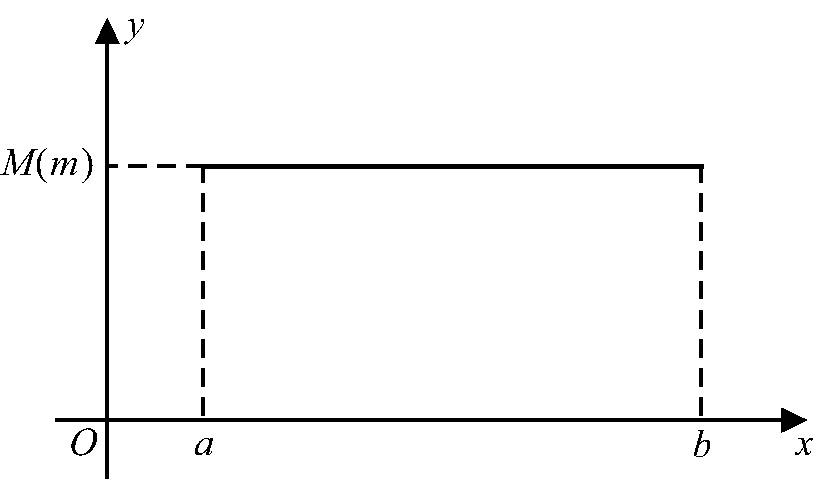
\includegraphics[width = 0.9\linewidth]{pic/C-2/Roll_1}
	\vspace*{-1em}
	\captionof{figure}{$M = m$时的函数图像}
	\label{Roll1}
\end{minipage}


(2)\enspace$M\geq m $\\
\noindent \circled{1} $M=f(a)=f(b)$.\\
\hspace*{2em} 如图 \ref{Roll2} 所示,当$M=f(a)=f(b)$时,由于$M>m$,那么$x_m\neq a,x_m\neq b$,即有$f(x)\geq f(x_m)$.由费马引理,得
\begin{equation}
	\nonumber
	f'(x_m)=0
\end{equation}
取$\xi=x_m$即可。

\begin{figure}[!htb]
\centering
	\begin{minipage}{0.49\linewidth}
		\centering
		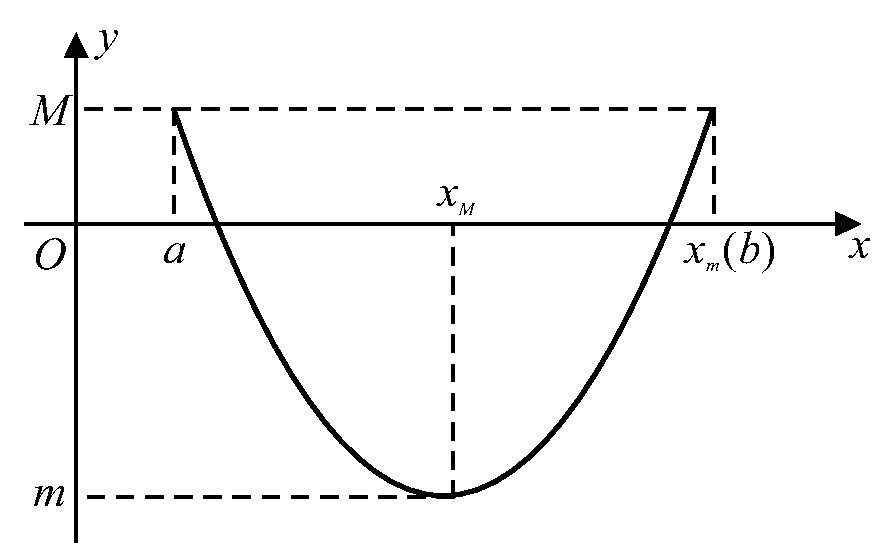
\includegraphics[width = 0.93\linewidth]{pic/C-2/Roll_3}
		\vspace*{-1em}
		\caption{$M = f(a) = f(b)$的函数图像}
		\label{Roll2}
	\end{minipage}
	\begin{minipage}{0.49\linewidth}
		\centering
		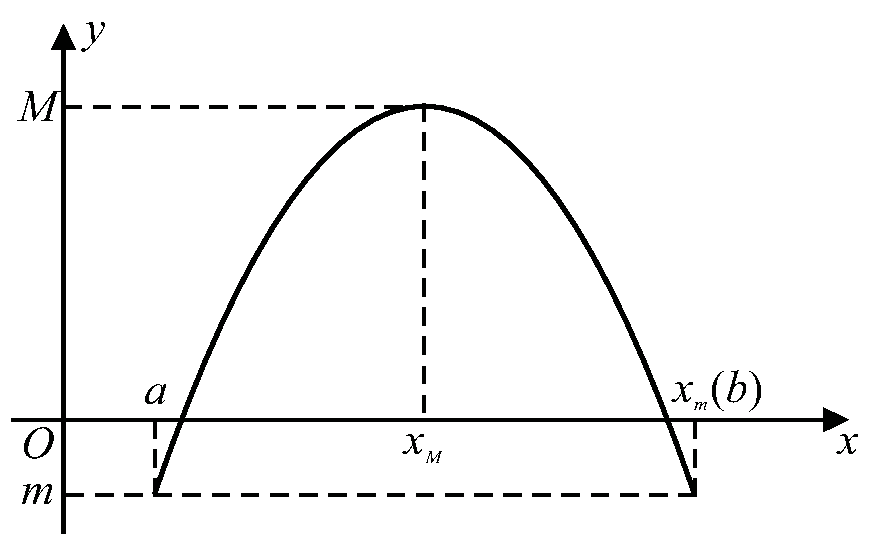
\includegraphics[width = 0.9\linewidth]{pic/C-2/Roll_2}
		\vspace*{-1em}
		\caption{$m = f(a) = f(b)$的函数图像}
		\label{Roll3}
	\end{minipage}
\end{figure}

\noindent \circled{2} $m=f(a)=f(b)$.\\
\hspace*{2em} 如图 \ref{Roll3} 所示,当$m=f(a)=f(b)$时,由于$M>m$,那么$x_M\neq a,x_M\neq b$,即有$f(x_M)\geq f(x)$.由费马引理,得
\begin{equation}
	f'(x_M)=0
\end{equation}
取$\xi=x_M$即可。

\noindent \begin{minipage}{0.6\linewidth}
\noindent \circled{3} $m<f(a)=f(b)<M$.\\
\hspace*{2em} 如图 \ref{Roll4} 所示,,当$m<f(a)=f(b)<M时$,$x_M,x_m\neq a,b.$.即有$f(x_M)\geq f(x)\geq f(x_m)$.那么由费马引理得
\begin{equation}
	f'(x_M)=0\hspace*{2em} f'(x_m)=0
\end{equation}
取$\xi=\big\lbrace x_M,x_m \big\rbrace$即可。	
\end{minipage}
\begin{minipage}{0.4\linewidth}
	\centering
	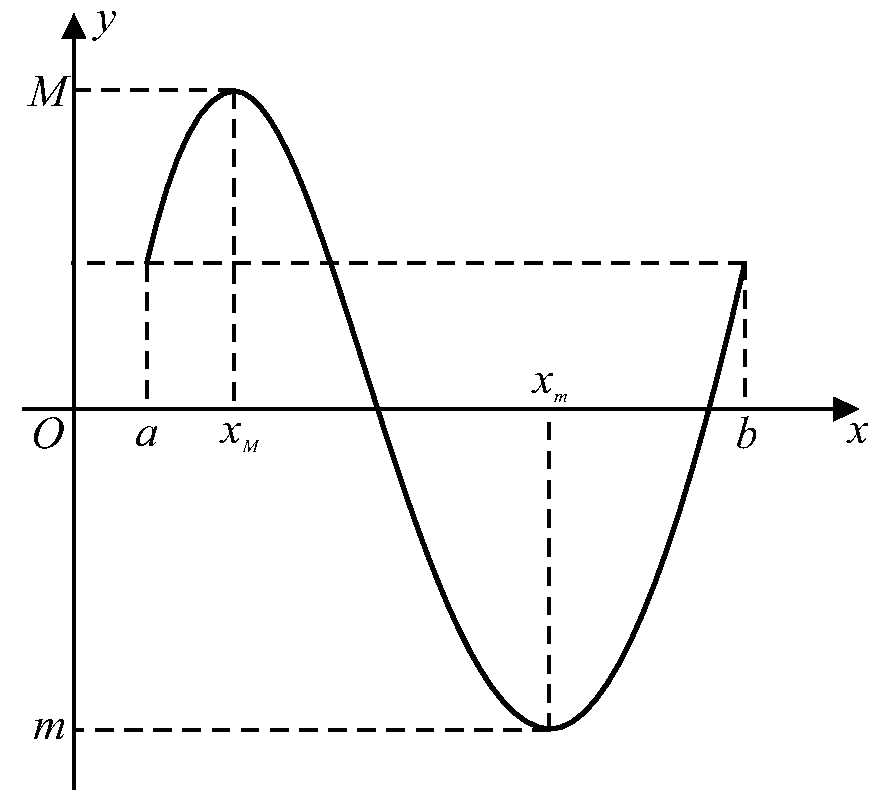
\includegraphics[width=0.95\linewidth]{pic/C-2/Roll_4}
	\vspace*{-1.5em}
	\captionof{figure}{$m < f(a) = f(b) < M$时的函数图像}
	\label{Roll4}
\end{minipage}

\subsection{拉格朗日中值定理}
罗尔定理中$f(a)=f(b)$这个条件是相当特殊的,它使罗尔定理的应用受到限制。所以我们将罗尔定理推广到拉格朗日中值定理.\\

\vspace*{-1em}
\theorem[拉格朗日(Lagrange)中值定理]

\noindent 设函数$f(x)$满足:
\\ \hspace*{2em}(1)\enspace 在闭区间$[a,b]$上连续;\\
\hspace*{2em} (2)\enspace 在开区间$(a,b)$内可导;\\
那么,在$(a,b)$内至少有一点$\xi(a<\xi<b)$使得
\begin{equation}
	\frac{f(b)-f(a)}{b-a}=f'(\xi)\vspace*{-1em}
\end{equation}

\noindent \proof 既然是罗尔定理的推广,我们想办法构造罗尔定理的条件,即函数的端点值相等。那么我们只需要将原函数减去直线(有向向量)$\bm{AB}$即可,如图 \ref{Lagrange} 所示。设直线$AB$的方程为
\begin{equation}
	\nonumber
	L(x)=f(a)+\frac{f(b)-f(a)}{b-a}(x-a)
\end{equation}
那么,我们构造一个辅助函数
\begin{equation}
	\nonumber
	F(x)=f(x)-L(x)=f(x)-f(a)-\frac{f(b)-f(a)}{b-a}(x-a)
\end{equation}
可以得到
\begin{equation}
\nonumber
	F(a)=f(a)-f(a)-\frac{f(b)-f(a)}{b-a}(a-a)=0-0=0
\end{equation}
从而,
\begin{equation}
	\nonumber
	F(b)=f(b)-f(a)-\frac{f(b)-f(a)}{b-a}(b-a)=f(b)-f(a)-[f(b)-f(a)]=0
\end{equation}
所以,$F(a)=F(b)=0$.由罗尔定理得,在$(a,b)$内至少有一点$\xi(a<\xi<b)$,使得$F‘(\xi)=0$.
\begin{equation}
	\nonumber
	F‘(\xi)=f'(\xi)-L‘(\xi)=f'(\xi)-\frac{f(b)-f(a)}{b-a}=0
\end{equation}
即\begin{equation}
	\nonumber
	\frac{f(b)-f(a)}{b-a}=f'(\xi)
\end{equation}

\begin{figure}[!htb]
	\centering
	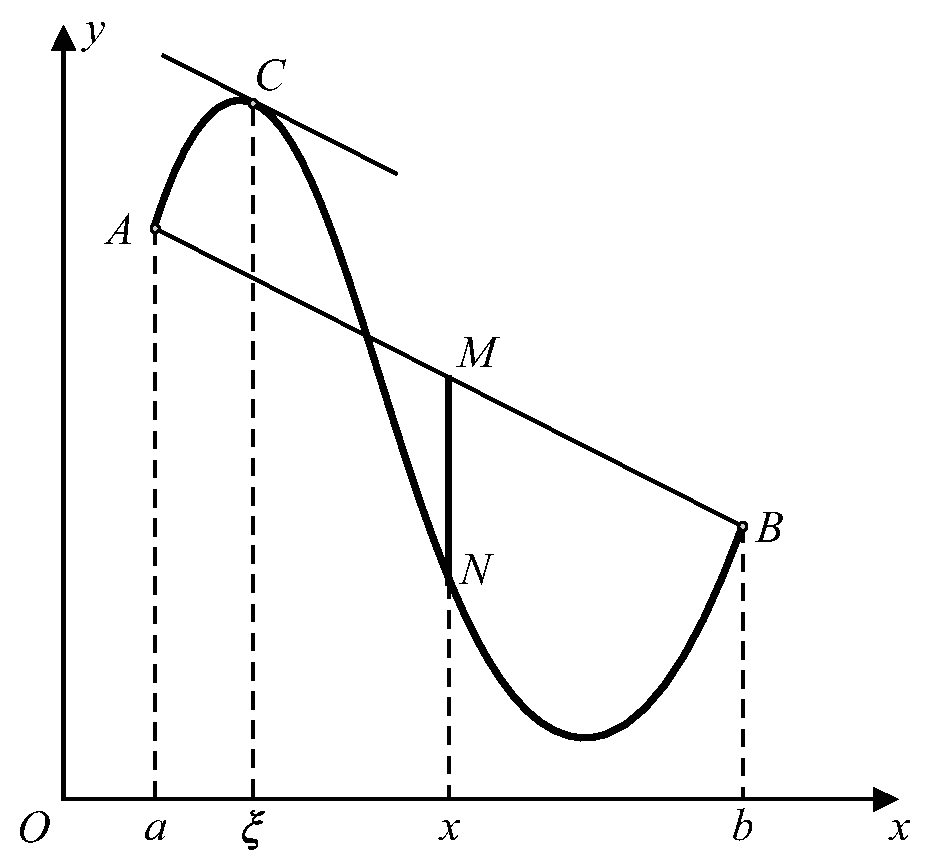
\includegraphics[width = 0.51\linewidth]{pic/C-2/Lagrange}
	\vspace*{-1em}
	\caption{拉格朗日定理的几何意义}
	\label{Lagrange}
\end{figure}

\vspace*{3em}
\myitem{\textbf{\normalsize 定理的几何意义}\vspace{0.5em}\\
\hspace*{2em} 如图 \ref{Lagrange} 所示,由于$\di\frac{f(b)-f(a)}{b-a}$代表的是函数端点连线$AB$的斜率,而$f'(\xi)$代表的是函数在点$C$处的切线斜率。\\ 
	\hspace*{2em} 那么,拉格朗日中值定理的几何意义为:如果连续函数$y=f(x)$的弧$\wideparen{AB} $上除端点外处处具有不垂直于$x$轴的切线,那么这弧上至少有一点$C$,使曲线在点$C$处的切线平行于弦$AB$.}

